\chapter{Cơ sở lý thuyết và các nghiên cứu liên quan}
\section{Tổng quan về căng thẳng tâm lý}
Căng thẳng tâm lý chính là một hiện tượng xảy ra thường xuyên trong cuộc sống hằng ngày. Với một người bị căng thẳng tâm lý, việc căng thẳng có thể làm cho người ấy cảm thấy bồn chồn và ảnh hưởng đến công việc hoặc căng thẳng này có thể là nguyên nhân để người này đạt được những mục tiêu đề ra. 

\subsection{Định nghĩa căng thẳng tâm lý}
Căng thẳng tâm lý, hay còn gọi là stress, là một phản ứng tự nhiên của cơ thể khi đối mặt với những áp lực, đòi hỏi hoặc thay đổi trong cuộc sống. Theo định nghĩa truyền thống, stress là một trạng thái căng thẳng, mệt mỏi về tinh thần và thể chất, gây ra bởi những yếu tố gây căng thẳng (stressors) như công việc, học tập, mối quan hệ, hoặc các sự kiện quan trọng trong cuộc sống \cite{stress_def}.

Hiện tại, khái niệm "stress" ngày càng trở nên phổ biến và được nhắc đến thường xuyên. Có nhiều lý do khiến từ khóa này trở nên nổi bật trong cuộc sống hiện tại như:
\begin{itemize}
    \item Thứ nhất, nhịp sống hiện đại ngày càng nhanh, đòi hỏi con người phải làm việc và học tập với cường độ cao chưa từng có. Áp lực từ công việc, học tập, cuộc sống cá nhân chồng chất lên nhau, khiến nhiều người cảm thấy quá tải dẫn đến sự căng thẳng \cite{Herbert}.
    \item Thứ hai, sự phát triển của công nghệ và mạng xã hội cũng góp phần gia tăng căng thẳng. Việc luôn kết nối với thế giới ảo, so sánh bản thân với người khác, và tiếp xúc với lượng thông tin khổng lồ mỗi ngày khiến nhiều người cảm thấy áp lực và lo lắng \cite{Lazarus}.
    \item Thứ ba, sự thay đổi nhanh chóng của xã hội cũng là một yếu tố góp phần làm tăng căng thẳng. Các vấn đề như mất an toàn, bất ổn kinh tế, dịch bệnh, và các biến động xã hội đều có thể gây ra căng thẳng cho con người \cite{student_life3, student_life4}.
\end{itemize} 
do những lý do đó, con người ở thời điểm hiện tại đối mặt với nhiều thách thức đến từ các rối hoạn tâm lý.

\subsection{Sự tác động của căng thẳng tâm lý và hành vi}
Về tác động của căng thẳng tâm lý đến hành vi con người, một số sự thay đổi hành vi có thể nhận diện rõ ràng như sau:
\begin{itemize}
    \item Căng thẳng tâm lý gây ra những biến đổi đáng kể về mặt tâm lý. Khi căng thẳng kéo dài, con người thường trở nên cáu gắt, dễ nổi nóng, khó kiểm soát cảm xúc. Với sự chịu tác động thời gian dài các yếu tố trên, người bị căng thẳng tâm lý có thể phải chịu đựng các rối loạn tâm lý như lo âu, trầm cảm, mất ngủ, gây ảnh hưởng nghiêm trọng đến chất lượng cuộc sống.
    \item Căng thẳng kích hoạt hệ thần kinh giao cảm, gây ra nhiều phản ứng sinh lý nhằm chuẩn bị cho cơ thể đối phó với tình huống nguy hiểm \cite{Youngjun, Alan}. Tim đập nhanh hơn, huyết áp tăng, hô hấp gấp, đổ mồ hôi, và nhiệt độ cơ thể tăng lên. Các hormone căng thẳng như cortisol được tiết ra với lượng lớn, làm tăng lượng đường trong máu cung cấp năng lượng cho cơ thể. Tuy nhiên, nếu tình trạng căng thẳng kéo dài, những phản ứng sinh lý này có thể gây hại cho sức khỏe.
    \item Căng thẳng cũng ảnh hưởng đến hành vi di chuyển của con người \cite{student_life2,student_life3, student_life4,eustress_distress4}. Một số người bị căng thẳng có thể có những hành vi tiêu cực như rối loạn giấc ngủ và rối loạn vận động \cite{eustress_distress4}. Những thay đổi này thường liên quan đến mức độ nghiêm trọng của căng thẳng và cách mỗi người đối phó với nó.
    \item Căng thẳng còn gây ra nhiều trở ngại cho khả năng làm việc và học tập \cite{stress_workload,eustress_distress3}. Khi căng thẳng, khả năng tập trung giảm sút, trí nhớ kém, khó khăn trong việc tiếp thu thông tin mới. Điều này dẫn đến giảm hiệu suất làm việc, sai sót trong công việc, và khó đạt được mục tiêu đã đề ra. Đối với học sinh, sinh viên, căng thẳng có thể gây khó khăn trong việc học bài, làm bài tập, và tham gia các hoạt động học tập khác dẫn đến sự chán nản và nguy cơ nghỉ học, bỏ lơ các bài tập, hạn nộp bài của học sinh, sinh viên ấy.
\end{itemize}

Từ những yếu tố trên, ta có thể thấy những tác động của stress lên hành vi con người trải dài nhiều lĩnh vực (tâm lý, hành vi, khả năng học tập làm việc). Vì vậy việc kịp thời nhận diện stress sẽ giúp ta có thể duy trì những tác động có lợi của stress cũng như hạn chế những tác động tiêu cực của quá nhiều căng thẳng đem đến. 
\subsection{Mặt tích cực và tiêu cực của căng thẳng tâm lý}
Trong giới khoa học, stress được chia làm hai loại eunstress và distress (căng thẳng tâm lý có lợi và căng thẳng tâm lý gây hại). Song việc nhận diện và đánh giá hai loại căng thẳng tâm lý này vẫn là một đề tài sôi nổi trong cộng đồng nghiên cứu về stress \cite{eustress_distress,eustress_distress2,eustress_distress3,eustress_distress4}. Một số nghiên cứu trong lĩnh này cho rằng có thể phân loại được căng thẳng có lợi và có hại dựa trên cường độ của sự căng thẳng song số khác lại phản bác điều đó. Nhưng chung quy lại các nghiên cứu vẫn công nhận sự hiện diện của stress có lợi và stress gây hại.
\subsection{Căng thẳng tâm lý có lợi}
 Căng thẳng tích cực, là một trạng thái tâm lý mang đến sự phấn khích. Do vậy, loại căng thẳng tâm lý này có khả năng tạo động lực giúp chúng ta tập trung hơn, sáng tạo hơn và tăng cường năng suất của cá nhân.

Một ví dụ điển hình về tác động của eustress đến trí nhớ được đề cập trong nghiên cứu của C. Sandi và M. T. Pinelo-Nava \cite{eustress_distress3}. Nghiên cứu của họ chỉ ra rằng, khi ở mức độ vừa phải, căng thẳng có thể cải thiện khả năng ghi nhớ và học hỏi thông tin mới. Điều này có nghĩa là, khi chúng ta cảm thấy hào hứng trước một bài kiểm tra quan trọng, chúng ta sẽ tập trung hơn vào việc ôn tập và ghi nhớ kiến thức.

Tóm lại, eustress đóng vai trò quan trọng trong việc thúc đẩy chúng ta phát triển và đạt được thành công. Tuy nhiên, để tận dụng tối đa lợi ích của eustress, chúng ta cần biết cách cân bằng giữa các loại căng thẳng và tìm ra những cách để quản lý stress hiệu quả.
\subsection{Căng thẳng tâm lý gây hại}
Distress, hay căng thẳng gây hại, là một trạng thái tâm lý gây ra cảm giác lo lắng, sợ hãi, và kiệt sức. Không giống như eustress, distress thường kéo dài và có thể gây ra nhiều hậu quả nghiêm trọng cho cả sức khỏe thể chất và tinh thần.

Một ví dụ về tác hại của distress là nghiên cứu của N. Schneiderman, G. Ironson, và S. D. Siegel\cite{eustress_distress4}. Trong bài báo "Stress and Health: Psychological, Behavioral, and Biological Determinants" (2005), các tác giả đã chỉ ra rằng mức độ căng thẳng cao kéo dài có thể làm suy yếu hệ miễn dịch, tăng nguy cơ mắc các bệnh mãn tính như tim mạch, tiểu đường,... \cite{eustress_distress4}

Cụ thể hơn, nghiên cứu đã cho thấy rằng stress mãn tính có thể gây ra các thay đổi sinh lý như tăng huyết áp, tăng mức cortisol (hormone căng thẳng)\cite{cortisol}, và làm suy yếu khả năng phục hồi của cơ thể sau khi bị bệnh. Điều này giải thích tại sao những người thường xuyên trải qua stress thường dễ bị ốm hơn và khó hồi phục hơn so với những người khác.

Vậy nên, distress không chỉ gây ra những khó chịu về mặt tâm lý mà còn có thể gây ra những hậu quả nghiêm trọng đối với sức khỏe thể chất.

% add more

\section{Internet kết nối vạn vật}
IoT, hay Internet Vạn Vật, là một mạng lưới bao gồm các thiết bị vật lý được nhúng với các cảm biến, phần mềm, và các công nghệ khác. Những thiết bị này có khả năng kết nối với nhau và trao đổi dữ liệu qua Internet. Chúng xuất hiênj ở khắp nơi trong cuộc sống hiện đại này có thể kể đến như những chiếc cửa ra vào thông mình, thiết bị đeo tay theo dõi sức khỏe cho đến các bóng đèn ngoài đường, tất cả đều có thể được kết nối vào mạng IoT.

Vì vậy ta có thể thấy công nghệ IoT đã và đang thay đổi cách chúng ta sống và làm việc. Trong lĩnh vực y tế, IoT giúp theo dõi sức khỏe cá nhân, cảnh báo sớm các vấn đề sức khỏe. Trong công nghiệp, IoT tối ưu hóa quy trình sản xuất, tăng năng suất và giảm thiểu lãng phí. Ngoài ra, IoT còn được ứng dụng rộng rãi trong các lĩnh vực như nông nghiệp thông minh, quản lý đô thị, giao thông vận tải, hoặc là quản lý năng suất, cảm xúc của con người.

Bên cạnh những sự ưu việt, IoT cũng đặt ra nhiều thách thức như vấn đề bảo mật thông tin, bảo vệ quyền riêng tư, và tiêu chuẩn hóa. Tuy nhiên, với sự phát triển của công nghệ, các vấn đề này đang dần được giải quyết. IoT hứa hẹn sẽ mang đến một tương lai thông minh và tiện lợi hơn, nơi mà mọi thứ đều được kết nối và tự động hóa. Đem lại cuộc sống tiện nghi nhất cho con người.

\section{Điện toán môi trường xung quanh}
Điện toán môi trường xung quanh (Ubiquitous Computing) là một khá niệm mới mô tả một môi trường nơi mà các thiết bị điện tử được tích hợp vào mọi vật dụng xung quanh chúng ta, tạo thành một mạng lưới kết nối thông minh. Điều này có nghĩa là bạn có thể tương tác với công nghệ ở bất cứ đâu, bất cứ lúc nào và thông qua bất kỳ vật thể nào. Với công nghệ này, con người trở thành trung tâm, xoay quanh là các yếu tương tác người - máy (HCI). Bằng cách xem con người là trung tâm này, các dữ liệu thu thập được sẽ phục vụ cho đời sống con người.

\begin{figure}[ht]
    \centering
    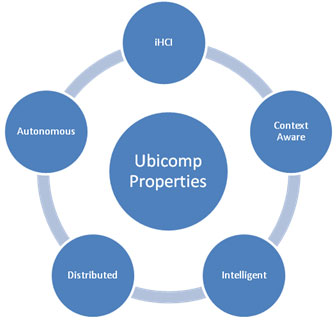
\includegraphics[width=0.5\linewidth]{Images/properties.jpg}
    \caption{ Điện toán môi trường xung quanh}
    \label{ubicomp}
\end{figure}

Cụ thể hơn, các công nghệ đang ứng dụng Ubiquitous Computing có thể kể tới như:
\begin{itemize}
    \item Phương tiện tự di chuyển: bằng cách tự động (Autonomous) xác định vị trí và các yếu tố liên quan của nhiều phương tiện và/ hoặc con người (Distributed), hệ thống điện toán môi trường xung quanh có thể nhận diện các đối tượng (con người, vật thể) với nhau (HCI). Sau đó tập trung nhận dạng các yếu tố liên quan (Context Aware), và sau đó có thể tối ưu hoá từng quyết định (Intelligent) của hệ thống.
    \item Nhà thông minh: bằng cách hiểu các thành viên trong nhà đang ở đâu (Distributed), hệ thống có thể tự động hoá thực hiện các tác vụ ở nhà (như mở máy điều hoà, bật đèn, mử cửa,...) tuỳ theo điều kiện thực tế để thuận tiện cho cuộc sống con người.
    \item Chẩn đoán tai nạn: đây là hướng phát triển ứng dụng của điện toán xung quanh được nói đến gần đây. Với những hệ thống "cảm biến" được con người mang theo hằng ngày (điện thoại, đồng hồ thông minh,...) việc nhận diện người đang bị tai nạn đã trở nên dễ dàng hơn.
    \item Chẩn đoán bệnh lý và sức khoẻ tâm thần: đây là ứng dụng của Ubiquitous Computing đang được đẩy mạnh trong giai đoạn hiện nay trong ngành y tế nói chung. Việc tận dụng các hệ thống cảm biến, camera xung quanh con người và những hệ thống đo lường dữ liệu của cá thể (điện thoại, máy tính bảng, đồng hồ thông minh,...) việc cảnh báo sớm nguy cơ mắc bệnh và nhận diện hành vi và sức khoẻ tâm thần của con người dần trở nên khả thi hơn.
\end{itemize}
Vì vậy có thể thấy công nghệ điện toán môi trường xung quanh đã được phổ biến ở thời điểm hiện tại, song khả năng tích hợp và tận dụng các tài nguyên này vẫn còn đang bị hạn chế.

\section{Tổng quan về học máy và trí tuệ nhân tạo giải thích}
Trong cuộc sống hiện đại, trí tuệ nhân tạo ngày càng được phát triển và ứng dụng trong thực tế. Theo sự phát triển của thế giới, trí tuệ nhân tạo ngày càng được tối ưu và có được khả năng hiểu và phân tích một cách logic. Sự phát triển này của trí tuệ nhân tạo ngày càng thúc đẩy sự phát triển của con người dẫn tới một viễn cảnh con người và máy có thể kết hợp thực hiện các việc con người chưa từng nghĩ là có thể.
\subsection{Lịch sử học máy}
Học máy, một nhánh của trí tuệ nhân tạo, ra đời với khát vọng tạo ra những hệ thống có khả năng học hỏi và tự cải thiện từ dữ liệu, giúp con người giải quyết được những vấn đề học búa. Ý tưởng này bắt nguồn từ mong muốn mô phỏng quá trình học tập của con người, nơi chúng ta rút ra bài học từ kinh nghiệm để đưa ra quyết định. Những năm 1950 đánh dấu bước khởi đầu khi các nhà khoa học bắt đầu nghiên cứu các thuật toán đơn giản (SVM, cây quyết định) cho phép máy tính nhận biết các mẫu trong dữ liệu. Tuy nhiên, do hạn chế về công suất tính toán và dung lượng dữ liệu, sự phát triển của học máy thời kỳ này còn khá khiêm tốn.

Sau một giai đoạn trầm lắng, học máy chứng kiến sự bùng nổ mạnh mẽ vào đầu thế kỷ 21. Sự gia tăng dữ liệu khổng lồ từ Internet và các thiết bị di động, cùng với sự phát triển của sức mạnh và tài nguyên tính toán, đã tạo điều kiện thuận lợi cho những đột phá trong lĩnh vực này. Các thuật toán học sâu (deep learning) dựa trên mạng thần kinh nhân tạo đã đạt được những thành công vượt trội trong nhiều lĩnh vực, từ nhận dạng hình ảnh đến xử lý ngôn ngữ tự nhiên, và đến giải thích được các sự vật hiện tượng trong cuộc sống của con người. Sự thành công của các ứng dụng học máy trong cuộc sống hàng ngày, như trợ lý ảo, xe tự lái, đã thúc đẩy sự đầu tư mạnh mẽ vào nghiên cứu và phát triển.

Do những điểm ưu việt của học máy đem lại, con người đã bước vào một kỷ nguyên mới, nơi mà con người có thể thu thập những phản hồi và gợi ý từ các hệ thống thông minh. những gợi ý và báo cáo này không những giúp con người kiểm soát được cuộc sống mình tốt hơn mà còn mở ra nhiều vùng đất mới cho con người khám phá về bản thân (như nhu cầu hiểu về bản thân, quản lý năng suất của bản thân,...)
% concept ML

\subsection{Học máy có giám sát}
Học máy có giám sát là một nhánh của trí tuệ nhân tạo, nơi các mô hình máy học được huấn luyện trên một tập dữ liệu lớn, mỗi dữ liệu đều được gắn một nhãn cụ thể. Giống như một đứa trẻ học hỏi từ những ví dụ thực tế, các mô hình này sẽ dần rút ra các quy luật, mối quan hệ giữa dữ liệu và nhãn để có thể đưa ra dự đoán chính xác cho dữ liệu mới.

Để thực hiện quá trình học và dự đoán, nhiều thuật toán khác nhau đã được phát triển có thể kể đến như: XGBoost, Random Forest và SVM.

Cụ thể hơn, XGBoost (hay Gradient Boosting)(tham khảo \cite{xgb,xgbNVIDIA}  và Hình \ref{XGBoost}) là một thuật toán mạnh mẽ, kết hợp nhiều mô hình đơn giản để tạo thành một mô hình phức tạp hơn. Nó có khả năng xử lý dữ liệu lớn và đạt được độ chính xác cao. Random Forest (tham khảo \cite{rf,rf_NVIDIA} và Hình \ref{rfNVIDIA}), cũng là một thuật toán tập hợp (hay Bagging), tạo ra nhiều cây quyết định khác nhau, sau đó kết hợp kết quả của chúng để đưa ra quyết định cuối cùng. Random Forest có khả năng giảm thiểu quá khớp và rất ổn định. Hơn thế, một thuật toán khác SVM, hay Support Vector Machine, tìm kiếm một đường phân cách tối ưu để phân loại dữ liệu. Nó thường được sử dụng khi dữ liệu có thể phân tách tuyến tính.
\begin{figure}[!ht]
    \centering
    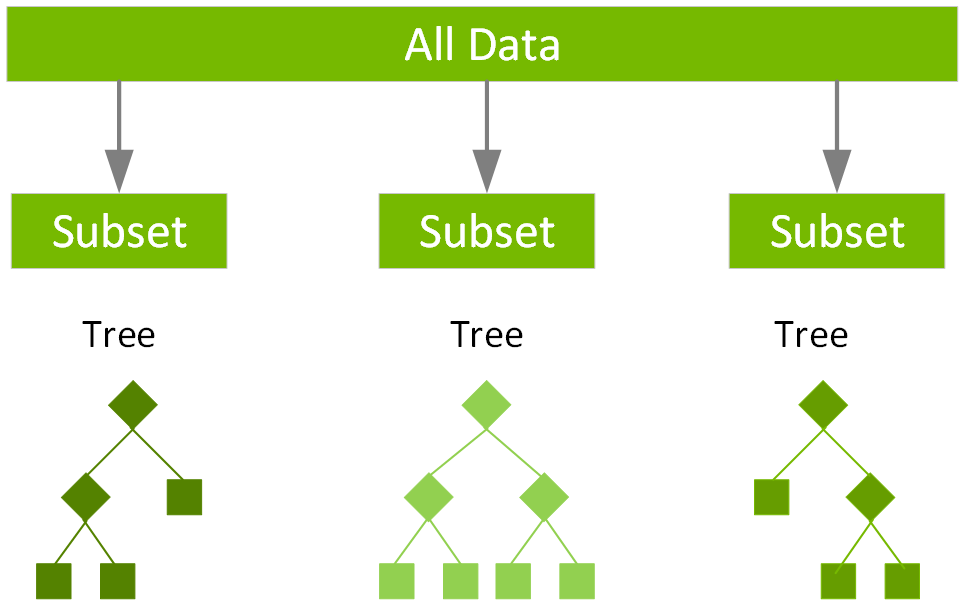
\includegraphics[width=0.8\linewidth]{XGboost.png}
    \caption{Hình ảnh minh hoạ cách phân cây quyết định của XGBoost (Nguồn NVIDA, \cite{xgbNVIDIA})}
    \label{XGBoost}
\end{figure}
\begin{figure}
    \centering
    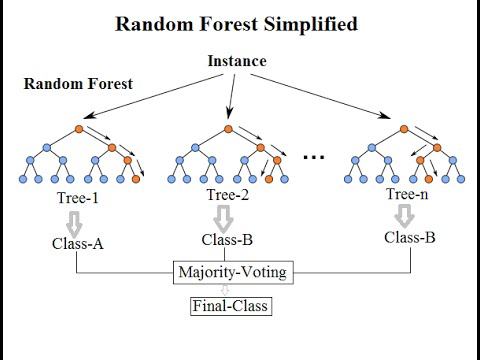
\includegraphics[width=0.8\linewidth]{rf.png}
    \caption{Hình ảnh minh hoạ cách phân cây quyết định của Random Forest (Nguồn NVIDA, \cite{rf_NVIDIA})}
    \label{rfNVIDIA}
\end{figure}
\subsection{Học máy không giám sát}
Nếu học máy có giám sát kể trển là quá trình máy tính học cách gán nhãn cho những dữ liệu có nhãn do ta gán sẵn, thì học máy không giám sát lại là một câu chuyện ngược lại. Ở đây, máy tính sẽ tự mình khám phá, tìm kiếm các mẫu ẩn, các cấu trúc tiềm ẩn trong dữ liệu mà không cần bất kỳ nhãn nào.

Một trong những nhiệm vụ phổ biến nhất của học máy không giám sát là clustering, hay còn gọi là phân cụm. Clustering giúp chia dữ liệu thành các nhóm (cụm) sao cho các điểm dữ liệu trong cùng một cụm có sự tương đồng cao, trong khi các điểm dữ liệu thuộc các cụm khác nhau lại khác biệt. việc phân cụm này giúp cho nhà nghiên cứu có thể quan sát rõ hơn cách hành vi của một hoặc nhiều nhóm dữ liệu có sự tương đồng từ đó hiểu hơn về các nhóm dữ liệu.

Về clustering, các thuật toán nổi trội có thể kể đến như kMEANS, DBSCAN, hoặc Gaussian Mixture Models (GMM). các  thuật toán này đã mở ra khả năng cho việc gom cụm dữ liệu phục vụ và phát triển cho ngành học máy nói chung.


\subsection{Học máy tăng cường}
Nếu ví học giám sát là máy được học dữ liệu qua nhãn dán sẵn, học không giám sát là máy tự tìm ra đặc trưng và gom cụm các dữ liệu có tính tương đồng, thì học tăng cường lại giống như phép thử và làm lại. Nói cách khác, mô hình học tăng cường không chỉ đơn thuần phân loại hay tìm kiếm các mẫu ẩn mà còn tương tác trực tiếp với môi trường. Mô hình sẽ thực hiện các hành động và nhận lại phần thưởng hoặc hình phạt (thông qua hàm nhận và giá cả (gain and loss function)) dựa trên kết quả của hành động đó. Qua quá trình thử và sai liên tục, mô hình sẽ học cách đưa ra những quyết định tối ưu để đạt được mục tiêu đã đặt ra.

\subsection{Học sâu}
khi nhắc tới học máy hiện đại, học sâu (hay Deep Learning) lấy được sự chú ý trong thời điểm gần đây. Lấy cảm hứng từ cấu trúc và chức năng của não người, mạng học sâu đã tạo và sử dụng các mạng thần kinh nhân tạo với nhiều lớp để học từ dữ liệu, tìm ra các đặc trưng phức tạp và đưa ra quyết định.

Với học sâu, mạng này có thể tạo thực hiện những công việc từ phân loại (CNN, RNN), gom cụm (NN-clustering) và cũng có thể học tăng cường (Deep Q-Networks (DQN)). Ngoài ra, học sâu còn có một khả năng ưu việt khác là trích xuất dữ liệu - một điều các giải thuật học máy thông thường không thể.

Vì vậy học sâu đang ngày càng mở rộng tầm ảnh hưởng trong thực tế và là công cụ được tin dùng hàng đầu trong kỷ nguyên này.

\subsection{Trí tuệ nhân tạo giải thích}
XAI (Explainable Artificial Intelligence) hay Trí tuệ nhân tạo có thể giải thích là một lĩnh vực nghiên cứu tập trung vào việc làm cho các hệ thống trí tuệ nhân tạo trở nên minh bạch và dễ hiểu hơn. Thay vì chỉ cung cấp kết quả cuối cùng, XAI cho phép chúng ta hiểu rõ quá trình ra quyết định bên trong của các mô hình AI. Điều này đặc biệt quan trọng đối với các hệ thống AI được sử dụng trong các lĩnh vực có liên quan đến an toàn, pháp lý và y tế, nơi mà sự tin tưởng vào các quyết định của AI là vô cùng cần thiết. XAI sử dụng nhiều kỹ thuật khác nhau để giải thích, từ việc đơn giản hóa các mô hình phức tạp đến việc tạo ra các bản trực quan hoá về cách các yếu tố đầu vào ảnh hưởng đến kết quả cuối cùng.

XAI mang đến nhiều ứng dụng thực tế quan trọng, đặc biệt trong việc giải thích các quyết định phức tạp của các mô hình AI. Như trong lĩnh vực tâm lý học, XAI có thể được sử dụng để giải thích tại sao một mô hình AI lại dự đoán một người nào đó có xu hướng mắc rối loạn tâm lý, hoặc trầm cảm, hay stress. Điều này giúp các nhà tâm lý học hiểu rõ hơn về quá trình ra quyết định của mô hình và từ đó đưa ra những đánh giá chính xác hơn về tình trạng của bệnh nhân. Ngoài ra, trong lĩnh vực thị giác máy tính (Computer Vision), XAI có thể được dùng để giải thích tại sao một mô hình lại xác định một vật thể trong hình ảnh là một con mèo chứ không phải một con chó, một khối u là lành tính chứ không phải ác tính,... Bằng cách làm rõ những yếu tố hình ảnh quan trọng mà mô hình dựa vào, chúng ta có thể đánh giá được độ tin cậy của kết quả và cải thiện hiệu suất của mô hình.

Do vậy XAI đang nổi lên như là một phương pháp hiện đại trong ngành kỹ thuật y sinh - nơi những kết quả cần có những lý giải chính xác cũng như những lý giải đó sẽ giúp con người có cái nhìn tổng quan về cuộc sống của chính bản thân mình.
\begin{figure}
    \centering
    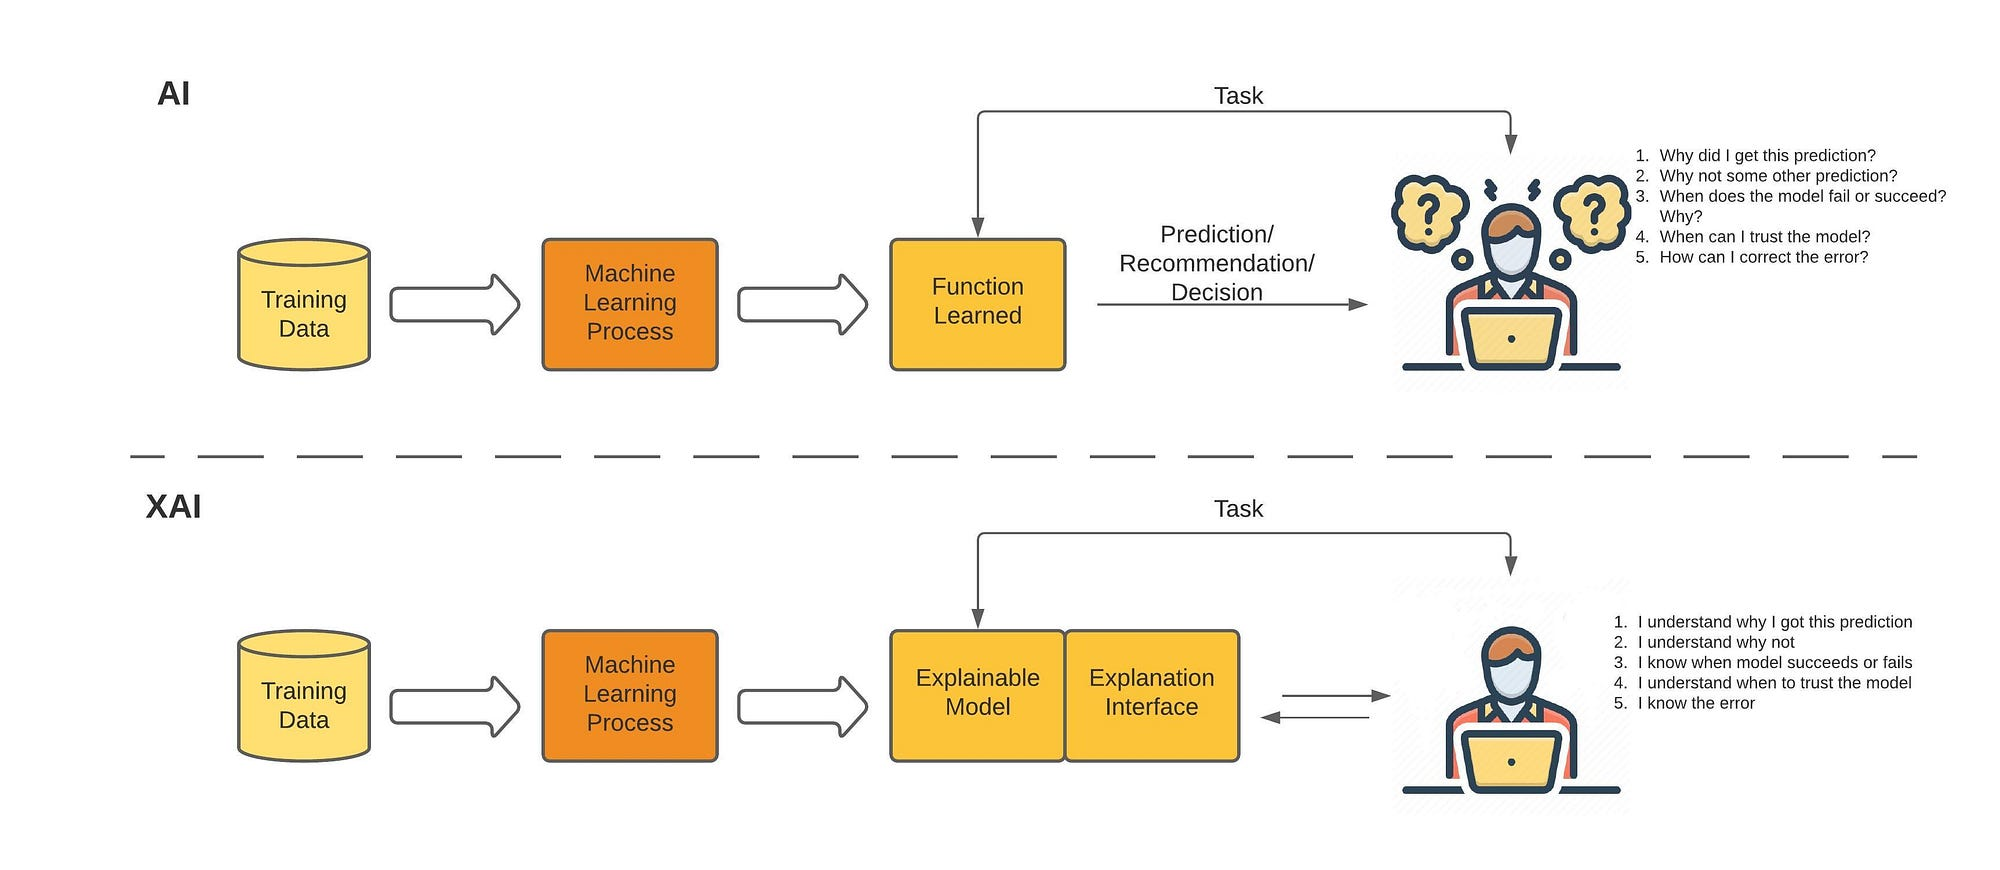
\includegraphics[width=\linewidth]{XAI.jpeg}
    \caption[]{So sánh cách hoạt động của mô hình AI truyền thống (trên) và XAI (dưới) (Nguồn Medium\footnotemark)}
    \label{fig:enter-label}
\end{figure}
\footnotetext{Understanding XAI and EBM truy cập từ: https://medium.com/predmatic/understanding-xai-and-ebm-112bcc7babc3}
\newpage
\section{Các nghiên cứu liên quan}
Căng thẳng tâm lý và tác động của căng thẳng tâm lý là một đề tài được quan tâm từ giới nghiên cứu  \cite{stress_heartrate,Stress_thermo,stress_eeg,student_life,student_life2,student_life3,student_life4,eustress_distress,eustress_distress2,eustress_distress3,eustress_distress4}. Với sự phát triển này, các vấn đề tâm lý đang có thể nhận diện bằng nhiều nguồn khác nhau: tín hiệu y sinh \cite{stress_eeg,stress_eeg2, stress_heartrate}, camera \cite{Stress_thermo}, tín hiệu điện thoại \cite{student_life, student_life2}. Việc này càng đẩy mạnh sự phát triển của công nghệ nhận diện sức khoẻ tinh thần, đưa ra những phương pháp nhận diện sức khoẻ tinh thần đáng tin cậy.
% add table of 
\subsection{Các nghiên cứu không sử sử dụng thiết bị di động}
NhTrong nhận diện sức khoẻ tinh thần, các tín hiệu y sinh là điều quan trọng để nhận diện được tình trạng tâm  lý của một đối tượng. Vì vậy nhóm nghiên cứu của Houtan \cite{stress_eeg} đã thực hiện đo tín hiệu điện não (EEG) của 11 tình nguyên viên trong công trường. Sử dụng các đặc trưng từ tín hiệu EEG theo miền thời gian, và miền tần số nghiên cứu này đã đạt được mô hình phân loại với độ chính xác cao (từ 60\% đến 80\%). Nhưng nhóm nghiên cứu này đề cập về vấn đề của sư suy giảm sư chính xác của việc nhân diên các diễn biến của tâm lý liên tục thông qua cửa sổ trươt (sliding window).

Về các nghiên cứu sử dụng tín hiệu y sinh, Salai và các cộng sự đã ứng dụng cảm biến nhịp tim đã có thể tạo ra mô hình phân loại stress tâm lý trên 46 tình nguyện viên với độ chính xác 75\% \cite{stress_heartrate}. Với mô hình này, nhóm của Salai sử dụng các yếu tố nhịp tim cổ điển như giá trị độ lệch chuẩn nhịp tim trung bình, nhịp tim trung bình, căn bậc hai trung bình của các chênh lệch liên tiếp (RMSSD) và PNN50 để làm đặc trưng của mô hình phân loại.

Về nghiên cứu dùng tín hiệu nhiệt hồng ngoại, Xiao và nhóm của mình đã thực hiện nghiên cứu trên tập dữ liệu bao gồm 32 sinh viên và học viên cao học \cite{Stress_thermo} trong môi trường có kiểm soát. Với ý tưởng stress sẽ gây tác động lên cơ thể, kích thích hệ thần kinh thực vật tạo phản ứng sinh mồ hôi và sẽ làm giảm cường độ hồng ngoại, nhóm đã tận dụng yếu tố sinh học này để thu thập các tín hiệu hồng ngoại này. Sau đó khi đưa các tín hiệu đầu vào này vào mô hình phân loại (Resnet) nhóm thu được kết quả khi chỉ sử dụng tín hiệu hồng ngoại độ chính xác của mô hình lên đến 76\%.

\subsection{Các nghiên cứu sử dụng thiết bị di động}
Để vượt qua các khó khăn về mặt nhận diện stress hằng ngày, các nhóm nghiên cứu \cite{student_life,student_life2,Muller,student_life4} đã đưa ra các cách để thu thập và nhận diện stress tâm lý trong tự nhiên có thể kể đến cụ thể như nhóm của Wang với đề tài StudentLife \cite{student_life}. Với dự án này nhóm đã thực hiện nghiên cứu trên 48 sinh viên tại đại học Dartmouth (Dartmouth College) về hành vi di chuyển thông qua định vị vệ tinh toàn cầu (GPS) và các yếu tố xoay quanh cuộc sống sinh viên. Nghiên cứu của nhóm gợi ý những đặc trưng về vị ví và ứng dụng mô hình cây quyết định để đánh giá các yếu tố về tâm lý cũng như học tập của sinh viên. Nghiên cứu này của Rui Wang chỉ ra rằng có thể giảm đến 63\% số lượng đặc trưng và đẩy nhanh tốc độ mô hình bằng việc chỉ xem xét các yếu tố được gợi ý của nhóm.

Vào năm 2022, nhóm của Wang phát triển trên hệ thống StudentLife khảo sát sự khác biệt của hành vi của sinh viên năm 1 và sinh viên các năm còn lại \cite{student_life4}. Ở nghiên cứu này, các đặc trưng về hoạt động thể chất, vị trí (bao gồm thời gian ở trong phòng ký túc xá cá nhân, ký túc xá của người khác, thời gian ở nhà ăn, tổng số địa điểm đến trong ngày,...), thời lượng sử dụng điện thoại, chất lượng giấc ngủ, và tính lặp lại của các đặc trưng được khảo sát kỹ. Về kết quả, nghiên cứu này chỉ ra được nhiều điểm khác biệt về hành vi của các sinh viên năm 1 với các sinh viên năm khác như: mức độ trầm cảm, mức độ stress, sự tham gia lớp học của sinh viên năm đầu và những sinh viên còn lại. Nghiên cứu này cũng chỉ ra rằng thời gian ở Greek house (một dạng nhà văn hoá dành cho sinh viên) và thời gian ở phòng ký túc xá của cá nhân là những thời gian quan trọng ảnh hưởng đến sức khoẻ tinh thần của sinh viên. Thế nhưng một hạn chế của nghiên cứu này là chưa thể hiện được lượng hoá được độ quan trọng của tất cả đặc trưng trích xuất, và chưa thể giải thích được lý do stress của từng sinh viên.

Một cách tiếp cận phát triển nghiên cứu \cite{student_life4} được nhóm của Muller đề xuất \cite{Muller} bằng cách xem xét thời gian ở nhà, số địa điểm đến, tổng quãng đường di chuyển, thời gian ở các địa điểm quan trọng, và thời gian di chuyển. Nhóm của Muller kết luận được thời gian ở nhà, và số địa điểm đến trong ngày mang ý nghĩa quan trọng đến sức khoẻ tinh thần. Hơn thế, nhóm cũng nêu lên sự cần thiết về việc hiểu các tác động của từng yếu tố lên sức khoẻ tinh thần của con người. Ngoài ra, bài nghiên cứu này cũng tập trung vào xu hướng di chuyển. Với việc khám phá xu hướng di chuyển, việc tìm ra các xu hướng của hành vi này sẽ giúp ta có thể kết nối sức khoẻ tinh thần và hành vi của con người.

Vào năm 2023, một nhóm nghiên cứu do Xu dẫn đầu đã phát triển từ mô hình của Wang, đã đưa lên một bộ dữ liệu là kết quả của sự kết hợp của 2 bộ dữ liệu về trầm cảm hiện có, đặt ra vấn đề mở rộng chủng tộc và đặt thách thức cho một hệ thồng toàn diện cho việc nhận diện stress\cite{student_life2}. Ở nghiên cứu này, nhóm xem xét các yếu tố vị trí, hoạt động điện thoại, di chuyển,... ở các buổi - điều các nghiên cứu trước chưa có nhiều sự quan tâm - để tìm ra đặc trưng dữ liệu. Về kết quả, nhóm đã đạt được độ chính xác phân loại stress vào khoảng 58\%, một sự phát triển đáng kể so với các nghiên cứu trước.


% Vào năm 2024, một nghiên cứu về tâm lý khác đã được thực hiện bởi Nepal thực hiện trong vòng 4 năm để nhận diện các vấn đề tâm lý của sinh viên đại học trước và sau COVID 19 \cite{student life3}. Nghiên cứu này đã chỉ ra được các sự khác biệt trong hành vi con người trước và sau đại dịch và gợi ý phương hướng cho các nghiên cứu thực hiện thu thập dữ liệu của người dùng để phát hiện cá trạng thái và đưa ra những ứng xử phù hợp

\subsection{Nghiên cứu ứng dụng trí tuệ nhân tạo giải thích}
Việc ứng dụng trí tuệ nhân tạo giải thích trong lĩnh vực tâm lý chưa được quá chú trọng. Song trong lĩnh vực nhận diện và giải thích căng thẳng, nhóm của Shikha \cite{Shikha} đã ứng dụng công nghệ này để giải thích cho mô hình phân loại của nhóm. Ở nghiên cứu này, 58 tín hiệu sinh học được sử dụng để chẩn đoán stress tâm lý. Bằng việc ứng dụng XAI, nghiên cứu này chỉ ra được XAI có khả năng giải thích tốt các đặc trưng thu thập được. 

\begin{longtable}{p{0.05\linewidth}  p{0.25\linewidth} p{0.3\linewidth} p{0.3\linewidth}}

\caption{Bảng biểu về tổng hợp các nghiên cứu liên quan}
\label{related_ửoks_summary_tab}
% \renewcommand{\arraystretch}{1.5}
\fontsize{13}{16}
\selectfont

\hline
 \textbf{ID} &\textbf{Tên công trình}  &\textbf{Phương pháp nghiên cứu}  & \textbf{Kết quả nghiên cứu} \\
\hline
\endfirsthead

\multicolumn{4}{c}%
{{\bfseries \tablename\ \thetable{} -- tiếp theo}} \\
\hline 
 \textbf{ID} &\textbf{Tên công trình}  &\textbf{Phương pháp nghiên cứu}  & \textbf{Kết quả nghiên cứu} \\
\hline 
\endhead
\hline
 \multicolumn{4}{r}{{Tiếp tục ở trang kế tiếp}} \\ 
\endfoot
\endlastfoot
\cite{stress_eeg}&EEG-based workers' stress recognition at construction sites& Thu thập tín hiệu EEG và biển đổi tín hiệu này theo miền thời gian và miền tần số& Mô hình phân loại có độ chính xác cao nhưng vẫn có những thách thức với việc nhận diện ở phương pháp cửa sổ trượt  \\
\cite{stress_heartrate} & Low-cost heart
rate sensor and mental stress detection using machine learning & Phân tích các yếu tố nhịp tim như nhịp tim, PP50,... & Độ chính xác mô hình nhận diện căng thẳng đạt 75\%  \\
        \cite{Stress_thermo} & Reading between the heat: Co-teaching body thermal signatures for non-intrusive stress detection & Phân tích biểu đồ quang cận hồng ngoại để nhận diện stress & Mô hình có độ phân loại có độ chính xác 76\%  \\
       \cite{student_life4}  & First-gen lens: Assessing men-
tal health of first-generation students across their first year at college using mobile sensing & Phân tích các yếu tố hành động của sinh viên & Tìm ra được mối liên hệ của các hành động trong ngày và căng thẳng tâm lý  \\
\cite{student_life2}&Globem: Cross-
dataset generalization of longitudinal human behavior modeling.&Nghiên cứu các hoạt động của sinh viên theo buổi& Độ chính xác phân loại được 58\% với mô hình mà nhóm công bố. So sánh thông số này với các nghiên cứu khác tại thời điểm đó.\\
\cite{Shikha}&Optimization of wearable
biosensor data for stress classification using machine learning and explainable ai& Thu thập các tín hiệu EDA, BVP, IBI sau đó lựa chọn các đặc trưng theo chiến thuật Thuật toán di truyền với thông tin tương hỗ (GA-MI) \cite{GAMI} để chọn đặc trưng sau đó huấn luyện và giải thích mô hình bằng XAI& Chứng minh XAI có thể giải thích mô quyết định của mô hình tương đối chính xác với thực tế và các công cụ thống kê khác.




\hline
% \textbf{class\_schedule} & The time student have to go to school in that day\\
% \hline
% \multicolumn{2}{l}{$^*$ The total time is calculated by $\sum_{i\subset S} \{time\ diffence\}_i$, and the std is calculated by $\sum_{i\subset S} \{time\ diffence\}_i$ with 
% }\\
% \multicolumn{2}{l}{S is the set of grouped features in a day}

\label{feature_type}

\end{longtable}
% (to be added more papers in this group :( )


% Do khả năng tinh chỉnh cục bộ và đưa ra giải thích cục bộ, LIME phù hợp với việc giải thích quyết định của mô hình nhận diện stress do khả năng xem xét 




